\renewcommand{\mapa}{Poglavja/Slike/kompleksnost/kompleksna grayscale 300}

\begin{figure}[H]
    \begin{subfigure}{0.32\linewidth}
        
\includegraphics[width=\linewidth]{\mapa/rez35Poisson.png}
        \caption{Rekonstrukcija na 0.35 znanih podatkih.}
    \end{subfigure}
    \hfill
    \begin{subfigure}{0.32\linewidth}
        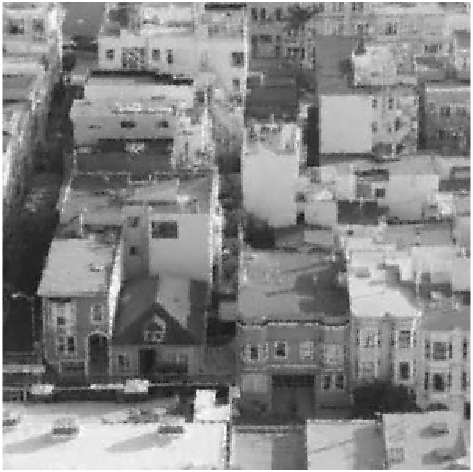
\includegraphics[width=\linewidth]{\mapa/rez45Poisson.png}
        \caption{Rekonstrukcija na 0.45 znanih podatkih.}
    \end{subfigure}
    \hfill
    \begin{subfigure}{0.32\linewidth}
        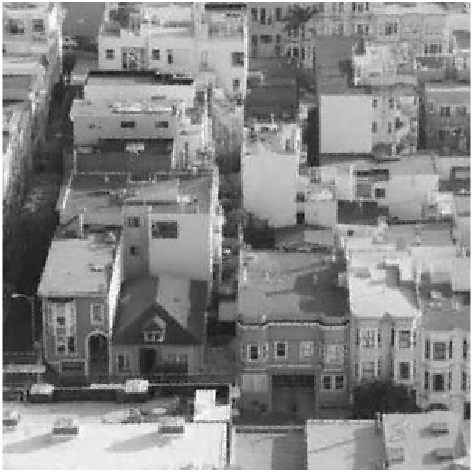
\includegraphics[width=\linewidth]{\mapa/rez60Poisson.png}
        \caption{Rekonstrukcija na 0.60 znanih podatkih.}
    \end{subfigure}
\end{figure}

\begin{figure}[H]
    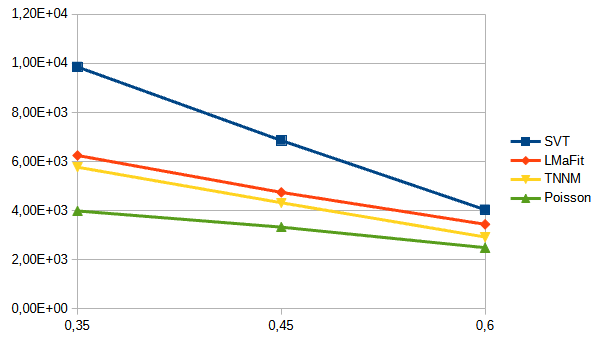
\includegraphics[width=\linewidth]{\mapa/napakaPoisson.png}
    \caption{Napaka rekonstrukcij slike mesta glede na delež znanih podatkov.}
\end{figure}

\begin{figure}[H]
    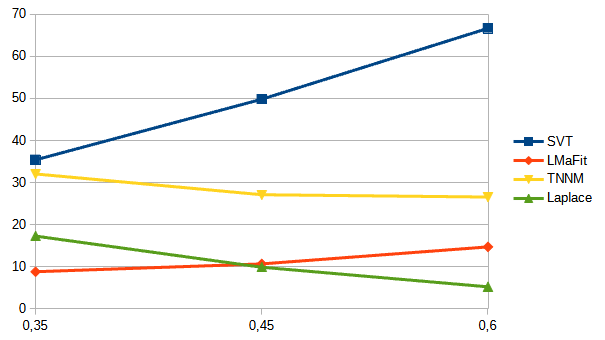
\includegraphics[width=\linewidth]{\mapa/casPoisson.png}
    \caption{Čas izvajanja rekonstrukcije slike mesta glede na delež znanih podatkov.}
\end{figure} 
